\chapter{Fundamentação Teórica}
\section{Ondas Gravitacionais}
\subsection{Introdução}

Qualquer objeto com massa exerce uma força de atração sobre outros objetos com massa, conhecida como “gravidade”. De acordo com a teoria da gravidade de Sir Isaac Newton \cite{newton1687philosophiae}, quaisquer dois objetos exercem uma atração gravitacional um sobre o outro de igual valor e sentido oposto, quando uma massa muda de posição, todo o campo gravitacional em todo o universo muda instantaneamente, e as forças gravitacionais resultantes são instantaneamente alteradas de acordo.

Mas a Teoria da Relatividade Geral de Einstein \cite{albert1920realtivity}, afirma que nenhuma informação pode viajar mais rápido que a velocidade da luz, incluindo informações sobre as posições de massa no universo, que são comunicadas através do campo gravitacional. A Relatividade Geral prevê que uma mudança no campo gravitacional viajará pelo universo à velocidade da luz e são exatamente essas mudanças no campo gravitacional que são as ondas gravitacionais.

De forma geral, as ondas gravitacionais podem ser pensadas como as ondas criadas quando jogamos pedras na superfície de um lago. Essas ondas são perturbações na geometria do próprio espaço-tempo emitidas por colisões violentas que acontecem no universo, que se propagam à velocidade da luz, carregando informações sobre suas origens, bem como pistas sobre a natureza da própria gravidade \cite{LSC-VIRGO, abbott2016observation, ramos2018teoria}.

\begin{figure}[ht]
\centering
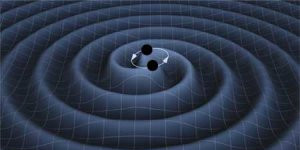
\includegraphics[width=.9\textwidth]{figuras/binary-wave_tn.jpg}
\caption{A impressão artística de ondas gravitacionais de dois buracos negros em órbita. [Imagem: T. Carnahan (NASA GSFC)]}
\label{fig:space-time}
\end{figure}

Ondas gravitacionais são criadas por massas móveis, da mesma forma que ondas eletromagnéticas são criadas por cargas em movimento. Mas como a gravidade é a mais fraca das quatro forças fundamentais (sendo as outras o eletromagnético, o nuclear fraco e o nuclear forte), as ondas gravitacionais são extremamente pequenas, produzindo um deslocamentos da ordem de \(10^{-18}\) metros, isto é, 1000 vezes menor que o diâmetro de um próton \cite{abbott2016observation}. Ondas dessa força serão produzidas por sistemas muito massivos que passam por grandes acelerações, como dois buracos negros em órbita que estão prestes a se fundir um com o outro. Como sistemas como esses são raros, essas fontes estarão a anos-luz de distância.

\subsection{Fontes e tipos de ondas gravitacionais}

Em geral, qualquer aceleração que não seja esfericamente ou cilindricamente simétrica produzirá uma onda gravitacional \cite{abbott2017gw170814}. Considere uma estrela que vai se transformar em uma supernova, esta explosão produzirá ondas gravitacionais se a massa não for ejetada de maneira esférica simétrica, embora o centro de massa possa estar na mesma posição antes e depois da explosão. Outro exemplo é uma estrela em movimento. Uma estrela perfeitamente esférica não produzirá uma onda gravitacional, mas sim uma estrela irregular \cite{abbott2017gw170817}.

Com base nessas diferentes fontes, os cientistas do LIGO definiram quatro categorias de ondas gravitacionais: Ondas Gravitacionais Contínuas, Ondas Gravitacionais de Sistemas Binários, Ondas Gravitacionais Estocásticas e Ondas Gravitacionais de colapso gravitacional. Cada categoria gera um conjunto único de "impressões digitais" ou assinaturas vibracionais características que os interferômetros do LIGO podem detectar e que os pesquisadores podem procurar nos dados do LIGO \cite{Christensen_2018}.

Ondas gravitacionais contínuas são produzidas por sistemas que têm uma frequência razoavelmente constante e bem definida. Exemplos disso são sistemas de estrelas binárias ou de buracos negros orbitando um ao outro ou uma única estrela girando rapidamente em torno de seu eixo com uma grande inchaço ou outras imperfeições na sua forma esférica. Espera-se que estas fontes produzam ondas gravitacionais comparativamente fracas, uma vez que elas evoluem ao longo de períodos de tempo mais longos e são geralmente menos catastróficas do que as fontes que produzem ondas gravitacionais de sistemas binários ou de colapso gravitacional \cite{beheshtipour2020deep}, Figura~\ref{figondacontinua}.

\begin{figure}[ht]
\centering
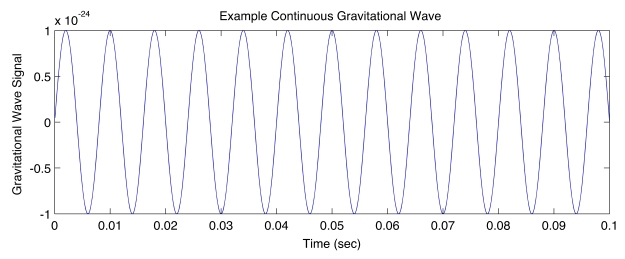
\includegraphics[width=.9\textwidth]{figuras/continuous_tn.jpg}
\caption{Um sinal de exemplo de uma fonte de onda gravitacional contínua. [Image: A. Stuver / LIGO]}
\label{figondacontinua}
\end{figure}

Ondas gravitacionais de sistemas binários são geradas durante o estágio final de vida de sistemas binários, onde os dois objetos se fundem em um. Esses sistemas são geralmente duas estrelas de nêutrons, dois buracos negros, ou uma estrela de nêutrons e um buraco negro cujas órbitas se degradaram até o ponto em que os dois objetos estão prestes a coalescer. À medida que os objetos giram em torno uma do outro, suas distâncias orbitais diminuem, retirando parte da energia orbital do sistema, enquanto suas velocidades aumentam \cite{Liu_2018}. Isso faz com que a frequência das ondas gravitacionais aumente até o momento da coalescência, Figura~\ref{figondainspiral}.

\begin{figure}[ht]
\centering
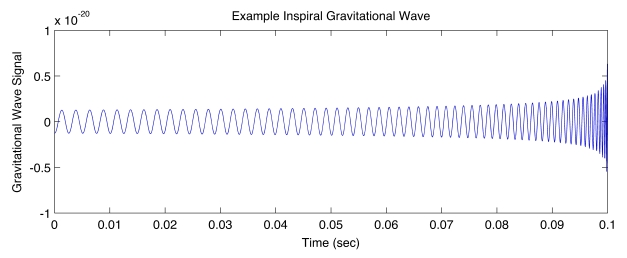
\includegraphics[width=.9\textwidth]{figuras/inspiral_tn.jpg}
\caption{Um sinal de exemplo de uma fonte de onda gravitacional de sistemas binários. [Image: A. Stuver / LIGO]}
\label{figondainspiral}
\end{figure}

As ondas gravitacionais de colapso gravitacional vêm de fontes desconhecidas ou imprevistas de curta duração. Há hipóteses de que alguns sistemas, como supernovas ou rajadas de raios gama, podem produzir ondas gravitacionais de colapso gravitacional, mas pouco se sabe sobre os detalhes desses sistemas para antecipar a forma que essas ondas terão \cite{Christensen_2018}, Figura~\ref{figondaruptura}.

\begin{figure}[ht]
\centering
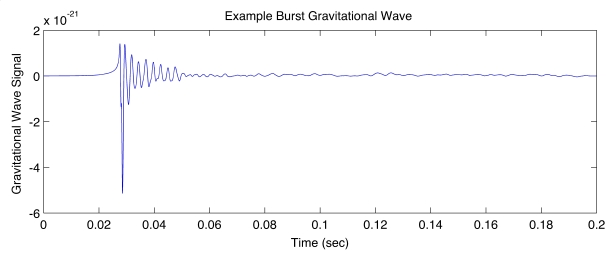
\includegraphics[width=.9\textwidth]{figuras/burst_tn.jpg}
\caption{Um sinal de exemplo de uma fonte de onda gravitacional de ruptura. [Image: A. Stuver / LIGO usando dados de C. Ott, D. Burrows e outros]}
\label{figondaruptura}
\end{figure}

Ondas gravitacionais estocásticas são as ondas gravitacionais relíquias da evolução inicial do universo. Assim como radiação cósmica de fundo em micro-ondas(Cosmic Micro-wave Background - CMB), que provavelmente é a luz residual do Big Bang, essas ondas gravitacionais surgem de um grande número de eventos aleatórios e independentes combinados para criar um fundo de ondas gravitacionais cósmicas. Essas pequenas ondas de todas as direções compõem o que é chamado de sinal estocástico, tendo um padrão aleatório que pode ser analisado estatisticamente, mas não previsto com precisão \cite{Christensen_2018}.

Espera-se que o Big Bang seja o principal candidato para a produção dos muitos processos aleatórios necessários para gerar ondas gravitacionais estocásticas e, portanto, podem conter informações sobre a origem e a história do universo \cite{Christensen_2018}, Figura \ref{figondaestocastica}.

\begin{figure}[ht]
\centering
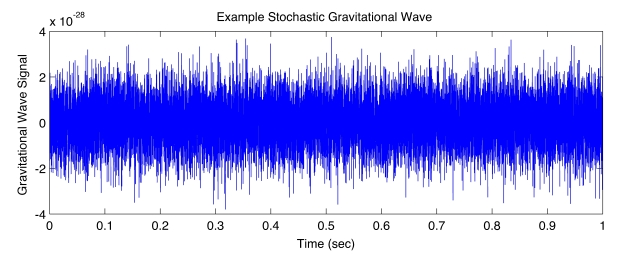
\includegraphics[width=.9\textwidth]{figuras/stochastic_tn.jpg}
\caption{Um sinal de exemplo de uma fonte de onda gravitacional estocástica. [Imagem: A. Stuver / LIGO]}
\label{figondaestocastica}
\end{figure}

\subsection{Equações de ondas Gravitacionais}

Uma maneira de se entender esse fenômeno matematicamente é através do cálculo que produz esse tipo de evento. Segundo a RG de Einstein, esses efeitos gravitacionais são descritos através da métrica $G_{\mu \nu}(x)$, que traz consigo informação acerca da curvatura do espaço-tempo.

Mas a equação de Einstein constitui um conjunto de 10 equações diferenciais parciais não lineares, o que, torna esse cálculo exaustivo e complexo. Uma maneira atrativa de se pensar nas equações de onda gravitacional produzidas por um sistema binário é tratar cada componente do sistema como um partícula. Segundo \cite{rubbo2007hands}, podemos fazer isto com a seguinte equação:

\begin{equation} \label{eqGW1}
\begin{split}
h(t) = \mathcal{A}(t)\cos \Phi(t),
\end{split}
\end{equation}

Na Equação \ref{eqGW1}, o $h(t)$ é a forma de onda gravitacional produzida pelos componentes(partículas) do sistema, também conhecida como deformação da onda gravitacional, $\mathcal{A}(t)$ é a amplitude dependente do tempo e $\Phi (t)$ é a fase da onda gravitacional. Ainda, segundo \cite{rubbo2007hands}, a amplitude $\mathcal{A}(t)$ pode ser expressa em termos dos parâmetros que caracterizam o sistema,

\begin{equation} \label{eqGW2}
\begin{split}
\mathcal{A}(t) = \frac{2(G\mathcal{M})^{5/3}}{c^4 r} \left(\frac{\pi}{P_{gw}(t)}\right)^{2/3} ,
\end{split}
\end{equation}
onde $G$ é a constante gravitacional de Newton, $c$ é a velocidade da luz, $r$ é a distância da luminosidade ao sistema binário e $P_{gw}(t)$ é o período da onda gravitacional. O valor $M \equiv (M_1 M_2)^{3/5}(M_1+M_2)^{-1/5}$ é a massa do \textit{chirp}\footnote{A massa do \textit{chirp} determina como o sistema evolui e o sinal de onda gravitacional emitido varia em amplitude e frequência, e é derivada da relação entre a massa total do sistema e a sua massa reduzida.} e comumente é usada na física das ondas gravitacionais, como uma escala de massa natural.

A fase das ondas gravitacionais, $\Phi (t)$, é análoga à fase para outro fenômeno das ondas, onde representa a localização do ciclo da onda que está colidindo com o detector no tempo $t$ e acompanha a evolução da amplitude da onda em função do tempo. A fase possui unidades de radianos e está relacionada à frequência da onda gravitacional $f_{gw}$ ou alternativamente ao período $P_{gw} = {f_{gw}^{-1}}$ pela integral da equação \ref{eqGW3}, onde, $\Phi_0$ é o valor da fase inicial, $\Phi_0=\Phi(t=0)$.

\begin{equation} \label{eqGW3}
\begin{split}
\Phi(t) = \Phi_0 + 2\pi \int_0^t \! \frac{{dt}^{'}}{P_{gw}(t^{'})}.
\end{split}
\end{equation}

Seguindo o exemplo dado em \cite{rubbo2007hands}, em que, os valores típicos da equação de amplitude de onda dado na Equação \ref{eqGW2}, foram substituídos por valores de um sistema binário de estrela de nêutrons localizado no centro de nossa galáxia, o mesmo afirma que as ondas gravitacionais são extremamente fracas e a amplitude de $\mathcal{A}$ é adimensional, portanto, a radiação gravitacional se manifesta na matéria ao induzir uma tensão. 

Em outros termos, a Equação \ref{eqGW1} proporciona a mudança relativa na distância entre dois pontos no espaço-tempo em função do tempo, tornando possível medir a separação entre duas massas e verificar se essas massas estão gerando uma onda gravitacional.

Como no eletromagnetismo, as ondas gravitacionais têm dois estados de polarização independentes designados por $\boldsymbol{+}$ e $\mathrm{X}$, como mostra a Figura \ref{figpolarization}. A polarização fornece, entre outras coisas, informação sobre a inclinação do plano orbital de um sistema binário em relação ao observador. Para um sistema binário, os dois estados são relacionados por uma mudança de fase de $90°$. Quando a linha de observação é paralela ao plano orbital do sistema, cada uma das componentes aparenta mover-se numa linha reta e neste caso possível, mostrar que a polarização das ondas gravitacionais emitidas será linear. 

\begin{figure}[ht]
\centering
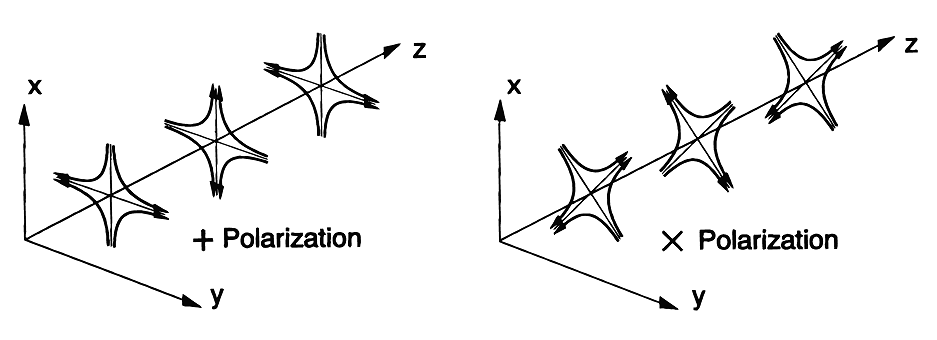
\includegraphics[width=.9\textwidth]{figuras/polarization.png}
\caption{Modos de polarização das ondas gravitacionais $\mathrm{h_{+}}$ e $\mathrm{h_{x}}$ propagando-se na direção $\mathrm{z}$. [Imagem: \cite{centrella2010black}]}
\label{figpolarization}
\end{figure}

Se, pelo contrário, a linha de observação for normal ao plano orbital, o movimento dos componentes será circular e a polarização observada será também circular. Entre estes dois casos limite existe uma gama de valores possível para a inclinação do plano orbital que pode em princípio ser deduzida através da polarização do sinal observado.

Consequentemente, a Equação \ref{eqGW1} captura a forma funcional dos dois estados de polarização. \cite{rubbo2007hands} afirma que ondas gravitacionais transportam energia e momento angular para longe do sistema binário, fazendo com que o período orbital diminua com o tempo, de acordo com

\begin{equation} \label{eqGW4}
\begin{split}
P_{orb}(t) = \left(P_0^{8/3} - \frac{8}{3}kt \right)^{3/8}
\end{split}
\end{equation}
onde $P_0$ é o período orbital no tempo $t = 0$, e $k$ é uma constante de evolução dada por:

\begin{equation} \label{eqGW5}
\begin{split}
k \equiv \frac{96}{5}(2\pi)^{8/3} \left(\frac{G\mathcal{M}}{c^3}\right)^{5/3}
\end{split}
\end{equation}

Como resultado do período orbital decrescente, os dois componentes binários se aproximaram lentamente, até o ponto em que colidem e coalesce em um único objeto remanescente, que ocorre quando $P_{orb}(t) = 0$.

Portanto, com a Equação \ref{eqGW1} é possível criarmos formas de ondas gravitacionais como mostra a Figura \ref{figmetade}. No entanto, é possível notar que a Equação \ref{eqGW1} não produz forma de onda, em que, o tempo é negativo, $P_{orb}(t) < 0$. Sendo assim, as formas de onda geradas por esse modelo não geram onda após a coalescência dos componentes. Devido a esta limitação este método de geração de ondas gravitacionais não será usado nesta pesquisa.

\begin{figure}[ht]
\centering
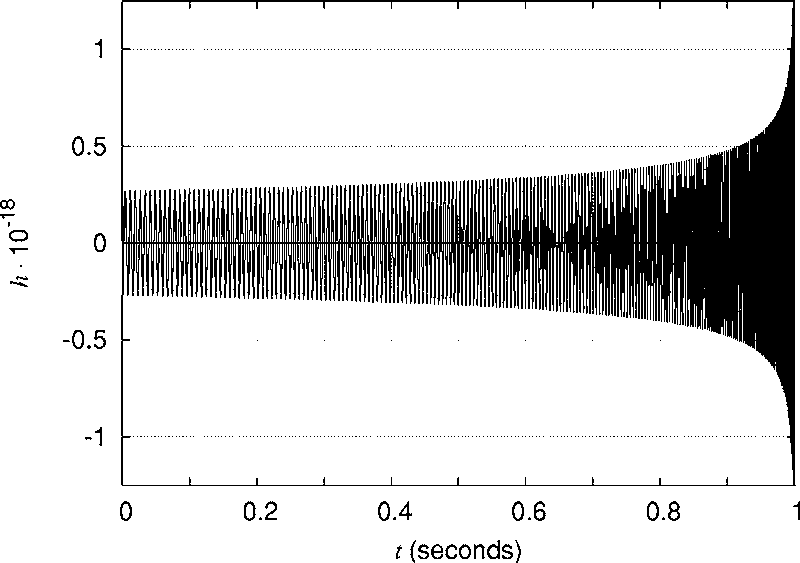
\includegraphics[width=.9\textwidth]{figuras/metade.png}
\caption{A forma de onda no último segundo antes da coalescência. Com a amplitude e a frequência do sinal aumentando com o tempo [Imagem: \cite{rubbo2007hands}]}
\label{figmetade}
\end{figure}

Esta é uma das maneiras que os astrônomos de ondas gravitacionais tem de extrair informações astrofísicas das formas de onda de sistemas binários observados. Claro que a análise de sinais reais é mais complexa. O principal desafio para a análise de dados reais é identificar o sinal oculto em um fluxo de dados com ruído. A abordagem mais comumente utilizada para esse problema na astronomia de ondas gravitacionais é usar a filtragem por coincidência. Se um sinal estiver presente em um fluxo de dados barulhento, o modelo fornecerá uma maneira de subtrair o ruído e deixar uma forma de onda limpa. Esta atividade assume que um modelo de sinal foi selecionado. Os astrônomos estimam os valores dos parâmetros astrofísicos que descrevem uma fonte de ondas gravitacionais a partir de formas de onda limpas \cite{rubbo2007hands}. 







\section{Redes Neurais Artificiais}

\subsection{Introdução às Redes Neurais Artificiais}

Qualquer que seja o organismo multicelular, independente da sua complexidade e organização, possui algum tipo de sistema nervoso que é responsável por alimentar o organismo através de entradas sensoriais sobre informações do ambiente em que o organismo vive. As informações coletadas são processadas e comparadas com experiências passadas e posteriormente são transformadas em ações apropriadas para a situação ou absorvidas em forma de conhecimento \cite{haykin1994neural}.

Para o organismo complexo, humano, o neurônio biológico é basicamente o dispositivo computacional elementar do sistema nervoso que possui muitas entradas e uma saída. As entradas ocorrem através das conexões sinápticas, que conectam a árvore dendrítica aos axônios de outras células nervosas. Os sinais que chegam por estes axônios são pulsos elétricos conhecidos como impulsos nervosos ou potenciais de ação, constituindo a informação que o neurônio processará de alguma forma para produzir como saída um impulso nervoso no seu axônio \cite{kovacs1996redes}. 

O cérebro humano possui uma capacidade incrível de absorção de conhecimento e é considerado o processador mais fascinante que existente, podendo desempenhar funções como percepção, intuição, inferência, reconhecimento de padrões, controle motor, entre outros. Ele possui cerca de $10^{11}$ de neurônios e cada neurônio pode receber de 1.000 a 10.000 contatos sinápticos em seu corpo e dendritos, que são responsáveis por todas as funções e movimentos do nosso organismo. Os neurônios estão conectados uns aos outros através de sinapses, e juntos formam uma grande rede, denominada Rede Neural, que proporciona uma fabulosa capacidade de processamento e armazenamento de informação \cite{kovacs1996redes}, Figura~\ref{figneuronios}. 

\begin{figure}[ht]
\centering
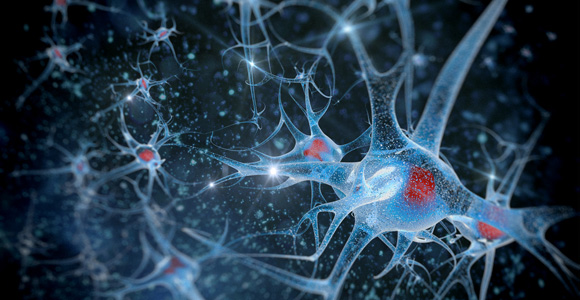
\includegraphics[width=1\textwidth]{figuras/axons.jpg}
\caption{Rede neural humana: o melhor processador de informações existente. [Imagem: \href{ https://neurogestion.wordpress.com}{ https://neurogestion.wordpress.com}]}
\label{figneuronios}
\end{figure}

\subsection{Redes Neurais Artificiais}

Há algumas décadas, surgiu a ideia de modelar, computacionalmente, as conexões neurais do cérebro humano, buscando reproduzir as características do neurônio biológico. Neste contexto, as redes neurais artificiais foram desenvolvidas, tomando-se como base as redes de neurônios cerebrais e sinapses biológicas do cérebro humano.

Uma rede neural é um sistema paralelo, distribuído, constituído pela interconexão de unidades básicas de processamento, denominadas neurônios artificiais, que têm a propensão natural para armazenar conhecimento experimental e torná-lo disponível para uso \cite{haykin2011neural}. Todo conhecimento adquirido pela rede se da através de um algoritmo de aprendizagem, cuja função é modificar os pesos de conexões entre os neurônios da rede, conhecidos como pesos sinápticos, de forma ordenada a fim de alcançar o mapeamento desejado.

\subsection{Neurônio Artificial}

A menor unidade básica de processamento de uma rede neural artificial é o neurônio, que recebe um sinal de entrada e produz um sinal de saída. O modelo de neurônio mais simples, comumente usado, e que engloba as principais características de uma rede neural biológica, paralelismo e alta conectividade, é o perceptron, representado na Figura~\ref{figperceptron}, que é composto por: m entradas (\(x_1, \ldots ,x_m\)), m pesos sinápticos (\(w_1, \ldots , w_m\)), uma variável de deslocamento linear \(b\) (do inglês: bias) e uma saída \(y\), descrito por:

\begin{equation} \label{eqRNA6}
\begin{split}
y = \theta(\sum_{i=1}^{m} x_i w_i + b)
\end{split}
\end{equation}

\begin{figure}[ht]
\centering
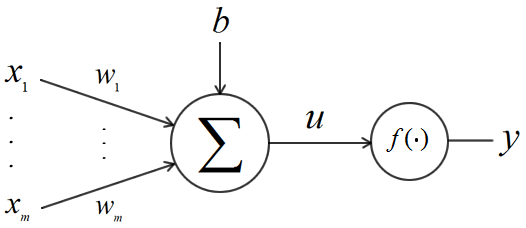
\includegraphics[width=.5\textwidth]{figuras/perceptron.png}
\caption{Modelo do neurônio artificial perceptron. [Imagem: \href{ http://computacaointeligente.com.br}{ http://computacaointeligente.com.br}]}
\label{figperceptron}
\end{figure}

A função \(\theta\) é conhecida como função de ativação ou função de transferência. Dentre as funções de ativação mais utilizadas estão a sigmoide e a tangente hiperbólica, definidas pelas equações abaixo, respectivamente \cite{articlefunclogtan}:

\begin{equation} \label{eq2}
\begin{split}
\theta(u) & = \frac{1}{1+ e^{-au}}\\
\theta(u) & = \frac{e^u - e^{-u}}{e^u + e^{-u}}
\end{split}
\end{equation}

\subsection{Arquitetura de uma RNA}

A arquitetura de uma RNA está relacionada com a maneira pela qual os seus neurônios estão organizados. De acordo com \cite{furtado2019redes}, as arquiteturas das RNAs são subdivididas em 3 classes: Rede Neural Feedforward de 1 camada, Rede Neural Feedforward Multicamadas e Redes Recorrentes ou Realimentadas. Além disso, a rede também é dividida em três tipos de camadas: a de entrada, a escondida e a de saída. 


As camadas podem ser classificadas em camadas de entrada, onde os padrões são apresentados à rede; camadas ocultas, onde é feita a maior parte do processamento; e a camada de saída, onde a conclusão do processamento é apresentada \cite{furtado2019redes}. Normalmente uma rede neural possui uma camada de entrada, uma camada de saída e \(k\) camadas ocultas, no qual \(k\) é definido empiricamente e varia de acordo com o problema.

Redes neurais do tipo Feedforward são redes de múltiplas camadas, ou seja, elas tem \(k\) camadas ocultas, no qual, a informação propaga-se da entrada para a saída, no caso, os sinais provenientes dos neurônios de uma camada só podem estimular os neurônios da camada seguinte. Quando a rede possuir todos os nós de uma camada comunicando-se com todos os nós da camada posterior, ela é dita totalmente conectada. Caso alguma das conexões sinápticas não esteja ligada com a camada subsequente, a rede é dita parcialmente conectada \cite{furtado2019redes}. A Figura \ref{figredeFeedforwardMulticamada} representa uma rede Feedforward multicamada de uma camada oculta totalmente conectada, ou seja, $k=1$.

% \begin{figure}[h]
% \centering
% 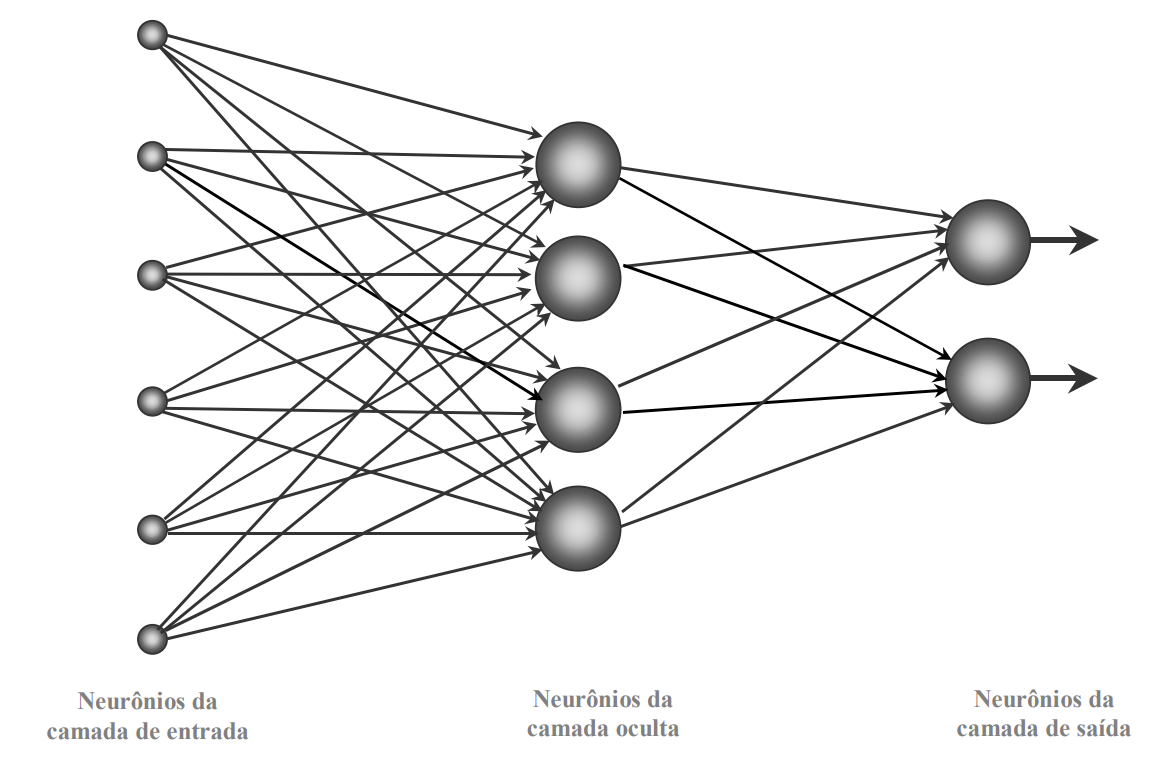
\includegraphics[width=.75\textwidth]{figuras/multicamadas.png}
% \caption{Exemplo de rede neural artificial do tipo Feedforward multicamadas. [Imagem: \cite{furtado2019redes}]}
% \label{figredeFeedforwardMulticamada}
% \end{figure}

\begin{figure}[h]
\centering
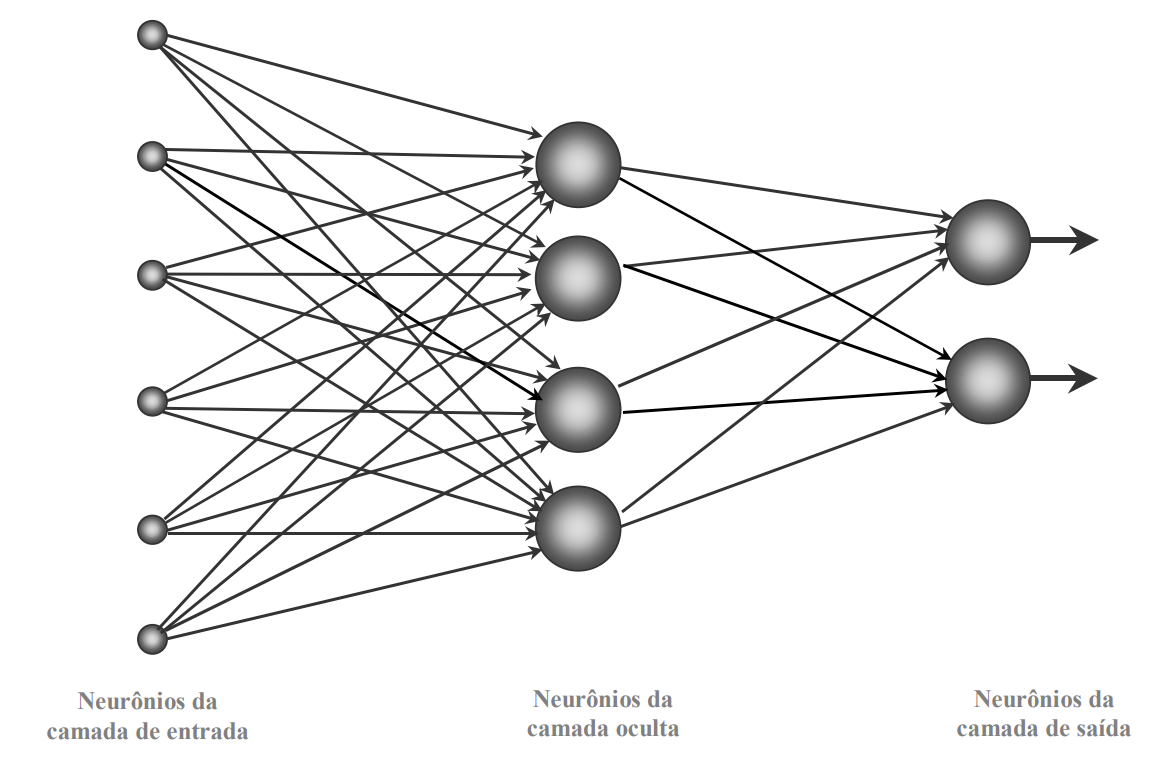
\includegraphics[width=.75\textwidth]{figuras/multicamadas.png}
\caption{Exemplo de rede neural artificial do tipo Feedforward multicamadas. [Imagem: \cite{furtado2019redes}]}
\label{figredeFeedforwardMulticamada}
\end{figure}

\subsection{Algoritmo de Treinamento}

A arquitetura da rede define, dentre outros parâmetros, a que tipo de treinamento a rede será submetida, capacitando-a a resolver o problema. No processo de treinamento a rede ‘aprende’ através de exemplos que relacionam as entradas e saídas do problema a ser solucionado. Essa abordagem é conhecida como aprendizado supervisionado. Dentre os algoritmos conhecidos, para solucionar esse tipo de problema, o mais utilizado é o backpropagation \cite{rumelhart1986learning}. A ideia do algoritmo é estimar os valores dos pesos e bias minimizando o erro entre a entrada e a saída desejada. O erro \(E\) cometido pela rede é calculado por:

\begin{equation} \label{eq3}
\begin{split}
E = \frac{1}{2} \sum_{i=1}^{p} \sum_{j=1}^{n} (d_{j}^{i} - y_{j}^{i})^2
\end{split}
\end{equation}
no qual, \(p\) é o número exemplos a ser utilizados no treinamento, n é o número de saídas da rede e, finalmente, \(d\) e \(y\) são as saídas desejadas e obtidas, respectivamente, para a entrada em questão.

Se o erro \(E\) encontrado for retropropagado (termo que foi derivado do nome do algoritmo backpropagation) pela rede, isto é, se o erro for propagado a partir da camada de saída até a camada de entrada, ela tentará estabelecer o quanto cada sinapse contribuiu para o erro, e este será usado para ajustá-las. A regra de atualização de cada peso sináptico da rede é calculado pela seguinte equação:

\begin{equation} \label{eqRNA4}
\begin{split}
W = W + \Delta W \therefore \Delta W = - \alpha\frac{\partial E}{\partial W}
\end{split}
\end{equation}

onde, \(\alpha\) é conhecido como taxa de aprendizado, que, resumidamente, indica o ‘tamanho do passo’ do gradiente rumo a minimização. O sinal negativo indica a busca por uma alteração no peso que reduza \(E\), sendo assim, quanto menor o erro, melhor a rede estará mapeando o problema.


% \subsection{Introdução às Redes Neurais Artificiais}

% A simulação cognitiva é uma técnica que permite imitar a forma e o comportamento de um organismo realizando suas atividades, estando inspirada em conceitos desenvolvidos na modelagem cognitiva, e utiliza os formalismos de representação de estruturas de domínio da Inteligência Artificial, que é um vasto campo que contém diversos componentes importantes, como as Redes Neurais Artificiais (RNAs) \cite{furtado2019redes}.

% Uma rede neural artificial (RNA) é basicamente um modelo computacional inspirado biologicamente. Ele tenta simular o processo de informação de um cérebro \cite{franchini2018artificial, yalccinreconfigurable}. Ele consiste em uma estrutura conexionista, na qual o processamento é distribuído por um elevado número de elementos processadores, os neurônios, amplamente interligados através de conexões com um determinado valor que estabelece o grau de conectividade entre estes, denominado peso da conexão ou sinapse e emula as propriedades decorrentes do alto grau de paralelismo e conectividade dos sistemas biológicos \cite{furtado2019redes}.

% Existem muitos tipos de RNA, mas, em geral, uma RNA é matematicamente um aproximador de função universal \cite{Cybenko1989}. Portanto, problemas com um alto número de observações e sem um modelo de análise conhecido são excelentes candidatos a sistemas baseados em soluções de RNA. Os recursos de generalização de informações e aprendizado da RNA são a base para gerar soluções para uma grande classe de problemas, como classificação, reconhecimento, clustering, previsão, regressão, mineração de dados, entre outros.

% \subsection{Histórico das Redes Neurais Artificiais}

% A primeira pesquisa relacionada ao desenvolvimento de um neurônio artificial biológico teve início na década de 40 do século passado, as primeiras informações sobre a neuro computação datam de 1943, em artigos de McCulloch e Pitts \cite{mcculloch1943logical}, que desenvolveram um modelo matemático de neurônio biológico artificial e sugeriam a construção de uma máquina baseada ou inspirada no cérebro humano, porém essa ideia não conseguiu desempenhar a tarefa de aprendizado.

% Desde então, pesquisadores começaram a desenvolver estudos relacionados com a forma de aprendizagem das redes biológicas e artificiais devido à experiência adquirida e sobre sua capacidade de executar determinadas funções (BRAGA et al., 2000).

% Em 1949 Donald Hebb escreveu um livro intitulado “A Organização do Comportamento” \cite{hebb1949organization}, onde apresentou uma hipótese a respeito da maneira com que a força das sinapses no cérebro se altera em resposta à experiência. Ele sugeriu que as conexões entre neurônios que são ativadas ao mesmo tempo tendem a se fortalecer, enquanto que as outras conexões tendem a se enfraquecer. Essa ideia fez dele o primeiro a propor uma lei de aprendizagem específica para as sinapses dos neurônios e esta hipótese passou a influenciar decisivamente na evolução da teoria de aprendizagem em RNAs, inspirando muitos outros pesquisadores a perseguirem a mesma ideia.

% Em 1951 foi construído primeiro neuro computador, denominado Calculadora Estocástica Neural-Analógica de Reforço (Stochastic Neural Analog Reinforcement Calculator - SNARC), por Mavin Minsky \cite{minsky1952neural}. Porem o SNARC nunca executou qualquer função de processamento de informação interessante. Somente mais tarde, em 1957 e 1958, que houve o primeiro desenvolvimento bem-sucedido de um neuro computador (Mark I Perceptron). Ele foi criado por Frank Rosenblatt, Charles Wightman e outros. Rosenblatt introduziu uma nova abordagem para o problema de reconhecimento de padrões com o desenvolvimento do Perceptron e também propôs um algoritmo para o ajuste dos pesos \cite{rosenblatt1958perceptron}.

% Por volta do mesmo período, Bernard Widrow, com a ajuda de alguns estudantes, desenvolveu um novo tipo de elemento de processamento de redes neurais chamado de Adaline (abreviação de Adaptive Linear Neuron ou posteriormente de Adaptive Linear Element) e mais tarde a sua generalização multidimensional, o Madaline (abreviação de Many ADALINE)\cite{widrow1960adaptive}. Esta rede era equipada com uma nova lei de aprendizado, conhecida como "Regra Delta", que depois foi generalizada para redes com modelos neurais mais elaborados, que diferente do Perceptron ainda permanece em uso \cite{furtado2019redes}.

% Os anos seguintes foram marcados por um entusiasmo exagerado criada pelos próprios pesquisadores desta área, que prometiam máquinas tão poderosas quanto o cérebro humano e que surgiriam em um curto espaço de tempo não acompanhada de resultados à altura, o que agravou a queda de financiamentos para as pesquisas e tirou a credibilidade dos estudos desta área \cite{furtado2019redes}.

% Em 1969, Minsky e Papert publicaram o livro “Perceptrons - An Introduction to Computational Geometry” \cite{minsky1969perceptrons}. Neste livro os autores explicam às limitações básicas das redes perceptrons, como por exemplo a impossibilidade de se implementar regras lógicas simples, como o ou-exclusivo. Neste livro os autores demonstraram que a rede perceptron, é capaz de executar as operações booleanas AND e OR, mas não é capaz de executar outras operações, como XOR (ou-exclusivo). Além do mais, os mesmos não acreditavam que uma arquitetura adequada em conjunto com um algoritmo de ajuste dos pesos pudesse ser desenvolvida de forma a superar este problema.

% Após a publicação deste livro as pesquisas na área de redes neurais paralisaram por um tempo. Os pesquisadores passaram a buscar por soluções em outras áreas, como da lógica matemática, que na época, encontrava-se em franca expansão, devido às grandes conquistas realizadas na área de computação \cite{nocaoderna}.

% Este período de pesquisa silenciosa perdurou até meados de 1982, com poucas publicações devido aos fatos ocorridos anteriormente. Entretanto, aqueles que pesquisavam nesta época como Teuvo Kohonen, Stephen Grossberg, B.Widrow, James Anderson, Edoardo Caianiello, Kunuhito Fukushima, Igor Aleksander e todos os que se seguiram no decorrer destes anos passaram a publicar diversas propostas para o desenvolvimento e para as aplicações de redes neurais, conseguindo assim, novamente estabelecer um campo concreto para o renascimento da área. O alto pode computacional, o desenvolvimento de novos algorítimos de aprendizado e o aprofundamento sobre a estrutura cerebral, foram os fatores que mais contribuíram para a retomada do interesse pela exploração das redes neurais artificiais \cite{nocaoderna}.

% Quando John Hopfield, renomado físico de reputação mundial e ganhador do Prêmio Nobel, se interessou pela neuro computação, ele incentivou e difundiu os princípios desta área entre importantes cientistas, matemáticos e tecnólogos altamente qualificados.

% Em 1986 o campo de pesquisa se extasiou com o desenvolvimento de um método para ajuste de parâmetros de redes não-recorrentes de múltiplas camadas. Este método, baseado em um algoritmo denominado retropropagação (backpropagation) \cite{rumelhart1986learning}, tornou-se largamente conhecido após a publicação do livro “Processamento Distribuído Paralelo” editado por David Rumelhart e James McClelland, fazendo com que pesquisadores das mais diferentes áreas passassem a visualizar interessantes aplicações para redes neurais artificiais.

% Desde então conferencias e institutos de pesquisa nesta área vem surgindo cada vez mais. E Recentemente, redes neurais artificiais tem se tornado a solução para muitas aplicações computacionais, tais como: reconhecimento de padrões, processamento de imagens, sistemas de controle, robótica, identificação de sistemas e astronomia.

% \subsection{Redes Neurais Biológicas}

% Qualquer que seja o organismo multicelular, independente da sua complexidade e organização, possui algum tipo de sistema nervoso que é responsável por alimentar o organismo através de entradas sensoriais sobre informações do ambiente em que o organismo vive. As informações coletadas são processadas e comparadas com experiências passadas e posteriormente são transformadas em ações apropriadas para a situação ou absorvidas em forma de conhecimento \cite{haykin1994neural}.

% Para o organismo complexo, humano, o neurônio biológico é basicamente o dispositivo computacional elementar do sistema nervoso que possui muitas entradas e uma saída. As entradas ocorrem através das conexões sinápticas, que conectam a árvore dendrítica aos axônios de outras células nervosas. Os sinais que chegam por estes axônios são pulsos elétricos conhecidos como impulsos nervosos ou potenciais de ação, constituindo a informação que o neurônio processará de alguma forma para produzir como saída um impulso nervoso no seu axônio \cite{kovacs1996redes}. 

% O cérebro humano possui uma capacidade incrível de absorção de conhecimento e é considerado o processador mais fascinante que existente, podendo desempenhar funções como percepção, intuição, inferência, reconhecimento de padrões, controle motor, entre outros. Ele possui cerca de $10^{11}$ de neurônios e cada neurônio pode receber de 1.000 a 10.000 contatos sinápticos em seu corpo e dendritos, que são responsáveis por todas as funções e movimentos do nosso organismo. Os neurônios estão conectados uns aos outros através de sinapses, e juntos formam uma grande rede, denominada Rede Neural, que proporciona uma fabulosa capacidade de processamento e armazenamento de informação \cite{kovacs1996redes}, Figura~\ref{figneuronios}. 

% \begin{figure}[ht]
% \centering
% 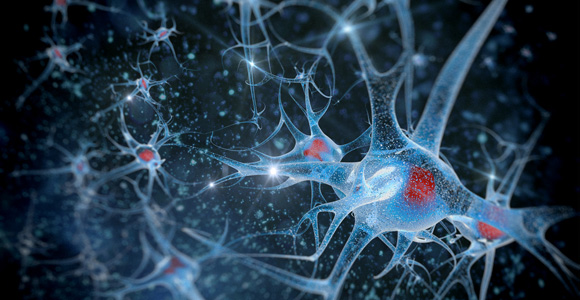
\includegraphics[width=1\textwidth]{figuras/axons.jpg}
% \caption{Rede neural humana: o melhor processador de informações existente. [Imagem: \href{ https://neurogestion.wordpress.com}{ https://neurogestion.wordpress.com}]}
% \label{figneuronios}
% \end{figure}

% O sistema nervoso é formado por um conjunto extremamente complexo de neurônios. Nesses, a comunicação é realizada através de impulsos. Quando um impulso é recebido, o neurônio o processa, e passado um limite de ação, dispara um segundo impulso que produz uma substância neurotransmissora o qual flui do corpo celular para o axônio que por sua vez pode estar ou não conectado a um dendrito de outra célula. O neurônio que transmite o pulso pode controlar a frequência de pulsos aumentando ou diminuindo a polaridade na membrana pós-sináptica. Eles têm um papel essencial na determinação do funcionamento, comportamento e do raciocínio do ser humano. 

% Ao contrário das redes neurais artificiais, redes neurais biológicas não transmitem sinais negativos, sua ativação é medida pela frequência (contínua e positiva) com que emite os pulsos. As redes neurais biológicas não são uniformes como as redes artificiais e apresentam uniformidade apenas em alguns pontos do organismo. Seus pulsos não são síncronos ou assíncronos, devido ao fato de não serem contínuos, o que as difere das redes artificiais. 

% Baseada na célula nervosa básica chamada neurônio, como qualquer célula biológica, o neurônio é delimitado por uma fina membrana celular que além da sua função biológica normal, possui propriedades que permitem a transmissão de sinais elétricos. A Figura \ref{figneuroniobiologico} ilustra a aparência de uma célula nervosa (neurônio) e de acordo  com  Braga  (2010,  p.  5),  em  uma  Rede  Neural  Biológica cada neurônio é dividido em três principais seções: o corpo do neurônio, os dendritos e o axônio.

% \begin{enumerate}[label={\alph*)}]
%     \item Dendritos: Tem por função, receber os estímulos transmitidos por outros neurônios;
%     \item Corpo do neurônio: Também chamado de soma, o qual é responsável por coletar e combinar informações vindas de outros neurônios. É o centro dos processos metabólicos da célula nervosa;
%     \item Axônio: Responsável pela condução do impulso nervoso na saída do neurônio.
% \end{enumerate}

% \begin{figure}[ht]
% \centering
% 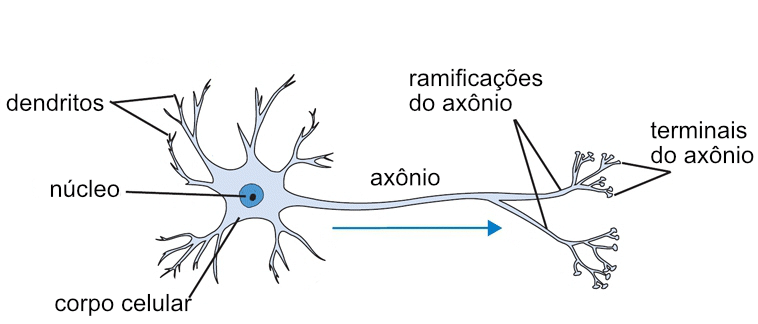
\includegraphics[width=1\textwidth]{figuras/neuronio.png}
% \caption{Representação de um neurônio biológico. [Imagem adapitada: \href{http://cs231n.github.io/neural-networks-1/}{http://cs231n.github.io/neural-networks-1/}]}
% \label{figneuroniobiologico}
% \end{figure}

% Na  Figura  \ref{figneuroniobiologico} é representado o neurônio biológico, onde os impulsos nervosos são receptados através dos dendritos que percorrem o núcleo envolvido pelo corpo do neurônio, passando pelo axônio até seus terminais para formarem as sinapses, que formam as interações entre os neurônios \cite{haykin2007redes}

% \subsection{Redes Neurais Artificiais}

% Há algumas décadas, surgiu a ideia de modelar, computacionalmente, as conexões neurais do cérebro humano, com intuito de emergir comportamentos inteligentes em máquinas. Neste contexto, surgiu as Redes Neurais Artificiais (RNA's), inspiradas na própria natureza das redes de neurônios cerebrais e sinapses biológicas.

% O trabalho em RNA's, comumente chamadas de “redes neurais” (RN), foi motivado desde o início pelo reconhecimento de que o cérebro humano computa de uma forma totalmente diferente do computador digital convencional. O cérebro é um computador altamente complexo, não linear e paralelo \cite{haykin2009neural}.

% Uma rede neural artificial é um sistema de processamento paralelo de informações constituído pela interconexão de unidades básicas de processamento, denominadas neurônios artificiais, que tem a propensão natural para armazenar conhecimento experimental e torná-lo disponível para o uso \cite{haykin2009neural}. Todo conhecimento adquirido pela rede se da através de um algoritmo de aprendizagem, cuja função é modificar os pesos de conexões entre os neurônios da rede, conhecidos como pesos sinápticos, de forma ordenada a fim de alcançar o mapeamento desejado.

% O neurônio artificial é a menor unidade de processamento de uma rede neural, que recebe sinais de entrada e produzem sinais de saída. O modelo de neurônio mais simples, e que engloba as principais características de uma rede neural biológica, paralelismo e alta conectividade, foi proposto por McCulloch e Pitts em 1943 \cite{mcculloch1943logical}

% O neurônio de McCullock e Pitts, apesar de simples, ainda é utilizado. Este modelo consistia basicamente em m terminais de entrada (dendritos) que recebem m valores \(x_1, \ldots ,x_m\) (que representam as ativações dos neurônios anteriores) e apenas um terminal de saída \(y\) (representando o axônio). As sinapses foram representadas por pesos (\(w_1, \ldots , w_m\)), acoplados nos terminais de entrada. Tais pesos podem possuir valores positivos ou negativos. Assim, o efeito da sinapse de um neurônio i pré-sináptico que emite um sinal \(x_i\) é \(w_{i}x_{i}\). O percentual de excitação de tal modelo é feito somando todas as sinapses correspondentes \(\sum w_{i}x_{i}\). 

% \begin{figure}[ht]
% \centering
% 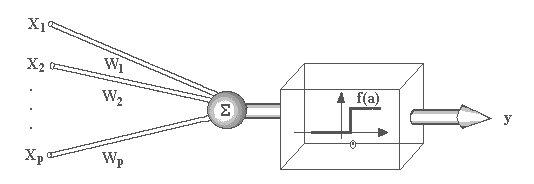
\includegraphics[width=1\textwidth]{figuras/Neuronio_McCulloch.png}
% \caption{Neurônio Artificial projetado por McCulloch e Pitts}
% \label{figneuronioMcCulloch}
% \end{figure}

% O disparo ou não do neurônio então se dá comparando o resultado dessa soma com o limiar de ativação, a partir de uma função de ativação. Por se tratar de um modelo binário, a saída do neurônio de McCulloch e Pitts pode ser pulso (1) ou não-pulso (0).

% Matematicamente o modelo apresentado na Figura \ref{figneuronioMcCulloch} pode ser representado por:

% \begin{equation} \label{eqRNA6}
% \begin{split}
% u_k = \sum_{j=1}^{m} w_{kj} x_i
% \\e
% \\ y_k = \theta(u_k)
% \end{split}
% \end{equation}

% A função de ativação, também conhecida como função restritiva, tem por objetivo limitar a amplitude do sinal de saída do neurônio. Para o modelo de McCulloch e Pitts, a função de ativação é a função de limiar, representada matematicamente como:

% \begin{equation} \label{eqRNA7}
% \begin{split}
% \theta(v) = \left\{ \begin{array}{rcl}1 & se & v\ge0
% \\ 0 & se & v<0
% \end{array}\right.
% \end{split}
% \end{equation}

% O modelo de McCulloch e Pitts pode ser esquematizado em uma forma mais geral de forma a possibilitar diversas aplicações: pode-se inserir um polarizador ou bias na entrada do neurônio e alterar a função de ativação \( \theta(·)\), utilizando para isso outras funções. O bias tem o efeito de aumentar ou diminuir a entrada líquida da função de ativação. Quatro elementos básicos podem ser identificados nesse modelo mais geral, a saber:

% \begin{enumerate}
%     \item Sinapses.
%     \item Somador.
%     \item Função de Ativação.
%     \item Bias (polarizador).
% \end{enumerate}

% O funcionamento do neurônio da Figura \ref{figneuronioMcCulloch}, acrescido do bias, pode ser descrito de forma matemática como:

% \begin{equation} \label{eqRNA8}
% \begin{split}
% y_k = \theta(u_k + b_k)
% \end{split}
% \end{equation}

% Este modelo se apresenta constante para quase todas as Redes Neurais, variando somente a função de ativação. Esta limita a amplitude do sinal de saída do neurônio. Normalmente a faixa de saída está em um intervalo fechado [0, 1] ou alternativamente em [-1, 1], podendo também este intervalo de saída estar entre (\(- \infty, + \infty\)) \cite{furtado2019redes}.

% \subsection{Funções de Ativação}

% Na equação \ref{eqRNA8}, a função de ativação processa o conjunto de entradas recebidas e o transforma em estado de ativação. Entre os diversos tipos de funções de ativação, as mais comuns estão representadas na Figura \ref{figfuncAtivação}. 

% \begin{figure}[ht]
% \centering
% 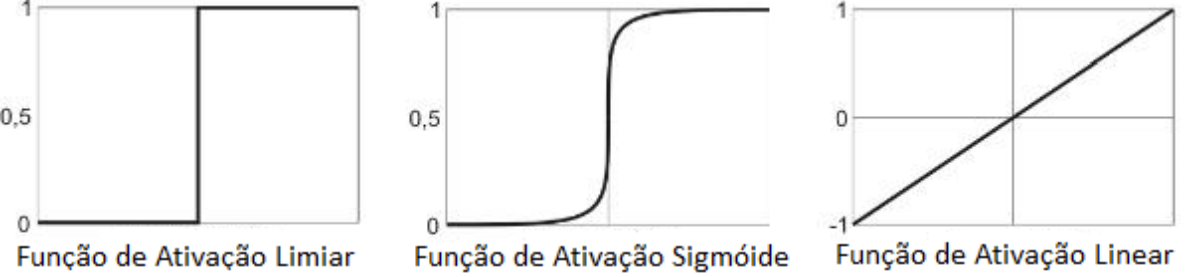
\includegraphics[width=1\textwidth]{figuras/funcAtivacao.png}
% \caption{Funções de ativação [Imagem adaptada: \cite{haykin1994neural}]}
% \label{figfuncAtivação}
% \end{figure}

% O tipo de função de ativação a ser utilizada é definido conforme a finalidade da construção da rede neural artificial. Permitir que a função de ativação assuma valores negativos pode trazer benefícios em alguns projetos e não trazer benefícios em outros.

% A função de ativação Limiar, utilizada no neurônio de McCulloch e Pitts, limita a saída do neurônio a apenas dois valores (binário: 0 e 1, ou bipolar: -1 e 1). Normalmente é utilizada em neurônios que tomam decisões binárias, como nos classificadores, definida como mostrado na equação \ref{eqRNA7}.

% A função de linear por partes e do tipo de função que pode ser visto como uma aproximação de um amplificador não linear, e possui a seguinte definição:

% \begin{equation} \label{eqRNA9}
% \begin{split}
% \theta(v) = \left\{ \begin{array}{rcl}1 & se & v\ge1/2
% \\ v & se & -1/2<v<+1/2
% \\ 0 & se & v<-1/2
% \end{array}\right.
% \end{split}
% \end{equation}

% Já a função Sigmoide é muito comum na construção de redes neurais artificiais e é utilizada por vários modelos de aplicações, apresenta um gráfico contínuo e suave, é monotônica e também diferenciável em qualquer ponto. A função Sigmoide pode ser representada pela função logística ou pela função tangente hiperbólica. Fundamentalmente, a diferença entre elas está nos intervalos nos quais são delimitadas. A função logística é definida pela equação \ref{eqRNA10}, onde o $b$ é o parâmetro de inclinação da função:

% \begin{equation} \label{eqRNA10}
% \begin{split}
% \theta(v) = \frac{1}{1+e^{-bv}}
% \end{split}
% \end{equation}

% Na função tangente hiperbólica, as funções de ativação definidas nas Equações \ref{eqRNA8}, \ref{eqRNA9} e \ref{eqRNA10} se estendem de $0$ a $+1$. Algumas vezes é desejável que a função de ativação se estenda de $-1$ a $+1$, assumindo neste caso uma forma anti-simétrica em relação à origem. Possui a seguinte definição:

% \begin{equation} \label{eqRNA11}
% \begin{split}
% \theta(v) = \tanh(v)
% \end{split}
% \end{equation}

% \subsection{Arquiteturas de Redes Neurais}

% % A maioria dos modelos de redes neurais possui alguma regra de treinamento, onde os pesos de suas conexões são ajustados de acordo com os padrões apresentados. Em outras palavras, elas aprendem através de exemplos (padrões).

% A arquitetura de uma rede neural está relacionada com a maneira pela qual os neurônios da mesma estão organizados. Em geral elas são subdivididas em 3 classes: Rede Neural Feedforward de 1 camada, Rede Neural Feedforward Multicamadas e Redes Recorrentes ou Realimentadas.

% A rede também é dividida em três tipos de camadas: a de entrada, a escondida e a de saída. As camadas de entrada e saída são intuitivas e representam o número de entradas e saídas do problema em questão. Já a escondida é a camada que fará a maior parte do processo de aprendizagem da rede. Normalmente uma rede neural possui uma camada de entrada, uma camada de saída e \(k\) camadas escondidas, no qual \(k\) é definido empiricamente e varia de acordo com o problema. 

% Redes neurais Feedforward (em português costumam traduzir como alimentação direta ou avante) apresenta uma organização similar à do córtex humano, em especial, a de 1 camada, em que, os neurônios se dispõem em camadas paralelas e consecutivas, e os axônios se estendem sempre no mesmo sentido, isto é, a informação propaga-se da entrada para a saída, não existindo portanto ligações entre os neurônios de uma mesma camada ou com camadas anteriores como pode ser visto na Figura \ref{figredeFeedforwardcamadaunica}, os nós da camada de entrada se comunicam diretamente com a camada de saída (nós computacionais). Suas principais aplicações são em memória associativa e no reconhecimento de padrões.

% \begin{figure}[ht]
% \centering
% 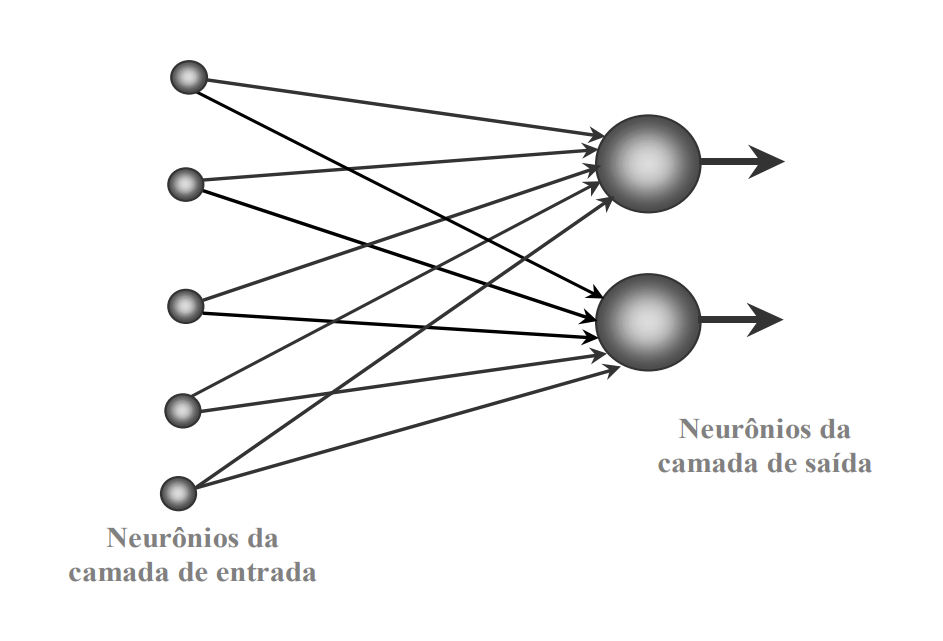
\includegraphics[width=.6\textwidth]{figuras/camada_unica.png}
% \caption{Exemplo de rede neural artificial do tipo Feedforward de 1 camada. [Imagem \cite{furtado2019redes}]}
% \label{figredeFeedforwardcamadaunica}
% \end{figure}

% Redes neurais do tipo Feedforward Multicamadas são redes de múltiplas camadas, ou seja, elas tem \(k\) camadas escondidas e seguem a mesma logica das redes de uma única camada, no caso, os sinais provenientes dos neurônios de uma camada só podem estimular os neurônios da camada seguinte, não existindo realimentação. Quando a rede possuir todos os nós de uma camada comunicando-se com todos os nós da camada posterior, ela é dita totalmente conectada. Caso alguma das conexões sinápticas não esteja ligada com a camada subsequente, a rede é dita parcialmente conectada. A Figura \ref{figredeFeedforwardMulticamada} representa uma rede Feedforward multicamada totalmente conectada. Suas principais aplicações são em reconhecimento de padrões, aproximador universal de funções e em controle.

% \begin{figure}[h]
% \centering
% 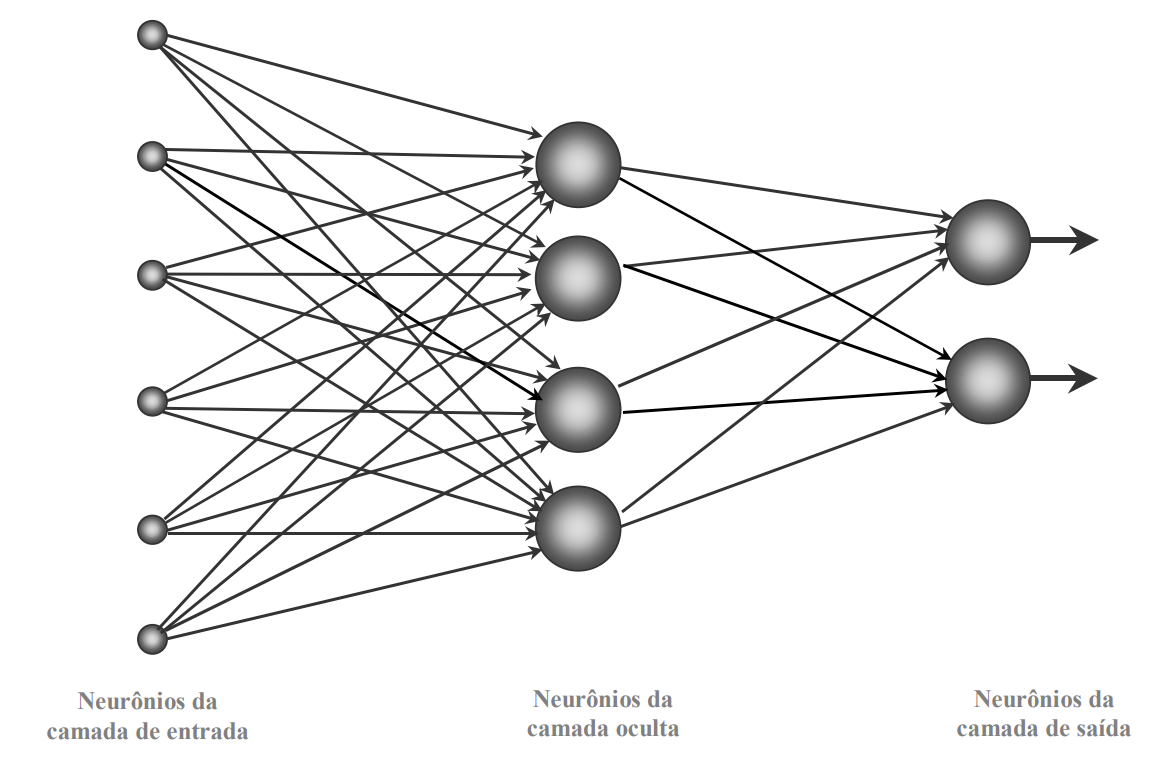
\includegraphics[width=.75\textwidth]{figuras/multicamadas.png}
% \caption{Exemplo de rede neural artificial do tipo Feedforward multicamadas. [Imagem: \cite{furtado2019redes}]}
% \label{figredeFeedforwardMulticamada}
% \end{figure}

% Redes Recorrentes ou Realimentadas distingue-se das redes neurais do tipo Feedforward por permitir a realimentação entre neurônios de camadas diferentes, ou ainda por fazer uma realimentação do neurônio com a sua própria saída (selffeedback). A Figura \ref{figredeRecorrente} apresenta uma rede recorrente com self-feedback e sem neurônios na camada intermediária. Suas principais aplicações são em sistemas dinâmicos, memória associativa, previsão e estimação, otimização e em controle, são mais poderosas que as outras, porém são bem mais complexas, tanto para utilização quanto para a análise dos resultados apresentados.

% \begin{figure}[ht]
% \centering
% 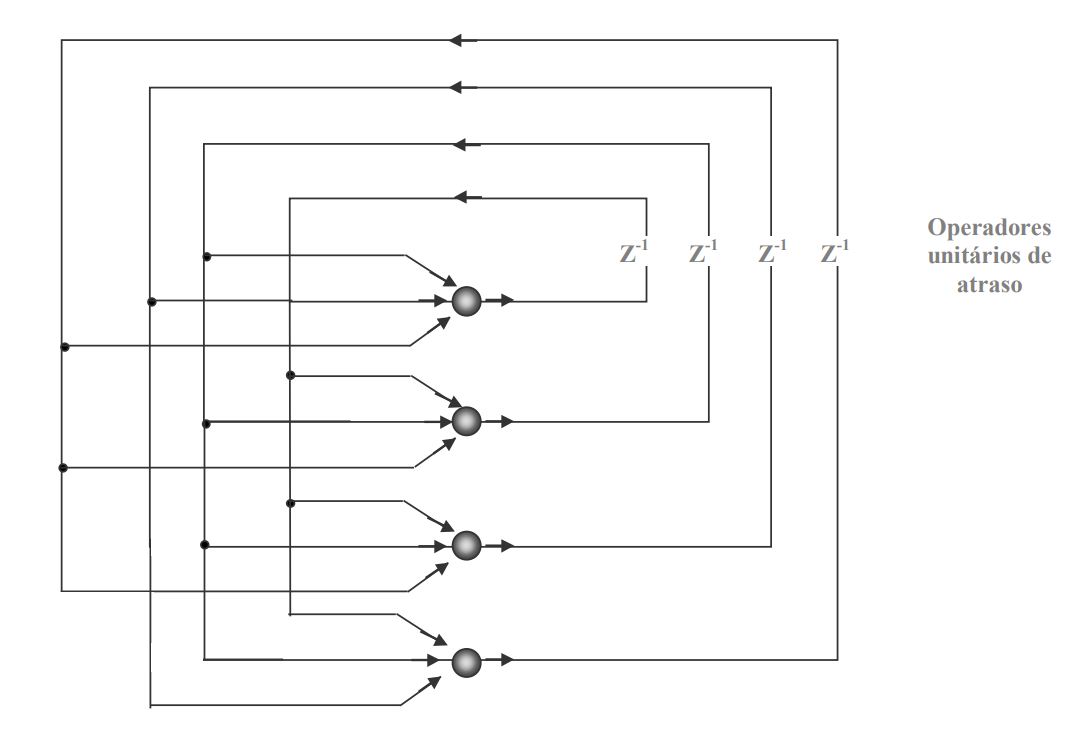
\includegraphics[width=.75\textwidth]{figuras/recorrente.png}
% \caption{Exemplo de rede neural artificial do tipo Recorrente ou Realimentada. [Imagem: \cite{furtado2019redes}]}
% \label{figredeRecorrente}
% \end{figure}

% \subsection{Treinamento}

% Após projetada a arquitetura da rede (determinar número de entradas, saídas, camadas escondidas e número de neurônios), é necessário um algoritmo de treinamento para realizar a aprendizagem da mesma. Para tal fim, é usualmente utilizada uma metodologia, em que a rede aprende acerca de seu ambiente a partir de um processo de ajustes sobre seus pesos sinápticos, isto é, os valores das sinapses são modificados aos poucos, visando minimizar os erros e otimizar a saída da rede. Idealmente, a rede se torna mais instruída sobre o seu ambiente após cada iteração do processo de aprendizagem \cite{haykin2011neural}.

% A arquitetura da rede define, dentre outros parâmetros, a que tipo de treinamento a rede será submetida, capacitando-a a resolver o problema. Segundo \cite{furtado2019redes}, os processos de aprendizagem podem ser agrupados em três paradigmas principais: aprendizado supervisionado, aprendizado não-supervisionado e aprendizado por reforço.

% Aprendizado supervisionado implica a existência de um supervisor ou professor, o qual é responsável por estimular as entradas da rede por meio de padrões de entrada e observar a saída da rede calculada pela mesma, comparando-a com a saída desejada

% O treinamento supervisionado utiliza um supervisor(professor), o qual é responsável por estimular as entradas da rede por meio de padrões de entrada e observar a saída da rede calculada pela mesma, comparando-a com a saída desejada. Através do erro, que é a diferença entre os valores esperados e os valores obtidos, o agente externo ajusta os parâmetros da rede. Este ajuste é feito até que o erro seja minimizado, passando a não existir mais ou atingindo um valor considerado satisfatório \cite{de2007redes}. 

% A partir deste momento, diz-se que a rede adquiriu conhecimento e apresenta-se treinada. Esse tipo de aprendizado é aplicado em problemas em que se deseja mapear padrões de entrada e saída. Dentre os algoritmos de treinamento supervisionado, pode-se citar como exemplo o do Erro Médio Quadrático e a generalização do mesmo, o backpropagation. Segundo \cite{haykin2011neural}, o backpropagation é o algoritmo de RNAs mais usado em aplicações práticas de previsão, classificação e de reconhecimento de padrões em geral. 

% No aprendizado não-supervisionado não existe um supervisor(professor) e em geral, apenas os padrões de entrada estão disponíveis, ou seja, não apresenta uma saída-alvo para comparação. Portanto, o processo de aprendizagem se dá pela existência de regularidades e redundâncias nos padrões de entrada apresentados à rede, a qual, deverá ser capaz de extrair as características relevantes dos impulsos, classificando-os em grupos pré-existentes. Esse processo se aplica em problemas que visam à descoberta de características estatísticas nos dados.

% O  aprendizado  por  reforço, mesmo  apresentando  similaridades  com  o  aprendizado supervisionado  e  não  supervisionado,  é  diferente,  pois  é  caracterizado  por haver  um supervisor que não indica uma saída desejada, apenas avalia se a saída está correta ou não. É um método baseado em tentativa e erro, pois os ajustes dos pesos a serem tomados irão depender unicamente das respostas produzidas pelo sistema durante o treinamento. O que o diferencia do treinamento supervisionado é que o supervisor sabe exatamente como ajustar os pesos no caso de erro.

% \subsection{Backpropagation}

% Este é um algoritmo de treinamento supervisionado para redes do tipo Feedforward
% que tenham neurônios com qualquer função de ativação que seja derivável. A ideia do algoritmo é estimar os valores dos pesos e bias minimizando o erro entre a entrada e a saída desejada usando o gradiente descendente. O erro \(E\) cometido pela rede é calculado por:

% \begin{equation} \label{eqRNA3}
% \begin{split}
% E = \frac{1}{2} \sum_{i=1}^{p} \sum_{j=1}^{n} (d_{j}^{i} - y_{j}^{i})^2
% \end{split}
% \end{equation}

% no qual, \(p\) é o número exemplos a ser utilizados no treinamento, n é o número de saídas da rede e, finalmente, \(d\) e \(y\) são as saídas desejadas e obtidas, respectivamente, para a entrada em questão.

% Se o erro \(E\) encontrado for retropropagado (termo que foi derivado do nome do algoritmo backpropagation) pela rede, isto é, se o erro for propagado a partir da camada de saída até a camada de entrada, ela tentará estabelecer o quanto cada sinapse contribuiu para o erro, e este será usado para ajustá-las. A regra de atualização de cada peso sináptico da rede é calculado pela seguinte equação:

% \begin{equation} \label{eqRNA4}
% \begin{split}
% W = W + \Delta W \therefore \Delta W = - \alpha\frac{\partial E}{\partial W}
% \end{split}
% \end{equation}

% onde, \(\alpha\) é conhecido como taxa de aprendizado, que, resumidamente, indica o ‘tamanho do passo’ do gradiente rumo a minimização. O sinal negativo indica a busca por uma alteração no peso que reduza \(E\), sendo assim, quanto menor o erro, melhor a rede estará mapeando o problema.
